\documentclass{article}
\usepackage{spconf,amsmath,amssymb,graphicx,booktabs,multirow,hyperref,xcolor,tabularx,tikz}
\usetikzlibrary{arrows.meta,positioning}
\hypersetup{hidelinks}

\newcommand{\method}{\textsc{ReIndexRepair}}
\newcommand{\fzero}{\ensuremath{F_0}}
\newcommand{\fone}{\ensuremath{F_1}}
\newcommand{\ftwo}{\ensuremath{F_2}}
% Generated from locked, human-adjudicated statistics.
\newcommand{\EvidenceBanner}{}
\newcommand{\SemanticFigureLead}{Human-adjudicated semantic evaluation}
\newcommand{\SubFlow}{94\!\to\!72\!\to\!71}
\newcommand{\SubPartialCount}{13/71}
\newcommand{\SubCompleteCount}{2/71}
\newcommand{\SubUnconditional}{15/94=16.0\%}
\newcommand{\SubRiskDifference}{15.5}
\newcommand{\SubRiskDifferenceCI}{7.0--23.9}
\newcommand{\SubPartialCI}{10.1--29.3}
\newcommand{\SubCompleteCI}{0.34--9.8}
\newcommand{\SubCompleteCIUpper}{9.8}
\newcommand{\SubHolm}{.0020}
\newcommand{\BoundaryFlow}{50\!\to\!20\!\to\!18}
\newcommand{\BoundaryPartialCount}{7/18}
\newcommand{\BoundaryCompleteCount}{1/18}
\newcommand{\BoundaryPartialCI}{17.3--64.3}
\newcommand{\BoundaryCompleteCI}{0.14--27.3}
\newcommand{\BoundaryUnconditional}{14/50=28.0\%}
\newcommand{\BoundaryHolm}{.0312}
\newcommand{\BoundaryMechanismSentence}{Independently of answer labels, migration occurs in 23/50 frozen constructions and 13/18 human-eligible cases; it accompanies 6/7 partial-arm recurrences.}
\newcommand{\AnnotationStatusParagraph}{Two independent humans labeled all 846 condition-blinded canonical outputs; 0 independent field decisions were \texttt{Unclear}, and a third person adjudicated 67 items. Raw agreement and three-class Cohen's $\kappa$ were target adoption 96.7\%/$\kappa=0.90$, correct adoption 96.0\%/$\kappa=0.92$, completeness 98.8\%/$\kappa=0.88$. Final labels contain 43 incomplete outputs, all retained in the reported flow.}
\newcommand{\PrimaryInferenceSentence}{Directional assignment of incomplete endpoints gives risk-difference ranges of substitution 5.6--21.1 points and boundary 16.7--38.9 points; neither least-favorable Holm test is significant ($p_{\mathrm{Holm}}=.9062/.9062$).}
\newcommand{\RepairFeasibleCount}{19/30}
\newcommand{\RepairCoverage}{63.3}
\newcommand{\RepairAbstainCount}{11/30}
\newcommand{\RepairActionSentence}{For feasible cases, the least-token choices are 3 all-attack, 6 sentence, 10 span, with median 4.0 and mean 17.5 edited tokens.}
\newcommand{\RepairFinalistCount}{19/19}
\newcommand{\RepairSelectedCorrect}{19}
\newcommand{\RepairDocumentCorrect}{10/30}


\title{REINDEXREPAIR: STATE-CONSISTENT EVALUATION OF POISON REPAIR IN RETRIEVAL-AUGMENTED GENERATION}

% ICASSP 2027 is not double blind. Author information is intentionally blank.
\name{\mbox{}}
\address{\mbox{}}

\begin{document}
\ninept % Official spconf option: 9 pt, with unchanged template margins.
\maketitle
\EvidenceBanner

\begin{abstract}
Deleting evidence in retrieval-augmented generation (RAG) need
not repair the rebuilt service: source edits may expose backup poison or migrate
residual text across chunks. We formalize this state mismatch as \emph{repair
mirage} and introduce \method{}, a materialized re-index protocol with exact
and provenance-complete controls. On frozen Natural Questions, target recurrence is \SubPartialCount{} after trace-visible
deletion versus \SubCompleteCount{} after complete-lineage removal (paired difference
\SubRiskDifference{} points; Holm-adjusted $p=\SubHolm$). A separate boundary mechanism yields
\BoundaryPartialCount{} versus \BoundaryCompleteCount{} ($p_{\rm Holm}=\BoundaryHolm$) in a boundary stress setting. In an exhaustive
30-incident oracle, \method{} finds a safety-and-correctness-preserving edit for
\RepairFeasibleCount{} cases; after four-way validation, exact-view finalist recall is
\RepairFinalistCount{}. This is an offline human-oracle analysis,
not a deployable selector. Under adjudicated labels, the results support
lineage-complete controls in these constructed settings; least-favorable
endpoint assignments retain positive differences but not statistical significance.
\end{abstract}

\begin{keywords}
retrieval-augmented generation, data poisoning, counterfactual evaluation,
re-indexing, information forensics
\end{keywords}

\section{Introduction}
Retrieval-augmented generation (RAG) couples language generation with external
evidence~\cite{lewis2020rag,karpukhin2020dpr}. PoisonedRAG shows that a few
injected passages can steer answers in million-scale corpora~\cite{zou2025poisonedrag}.
Removing evidence behind one failure, however, need not repair the next execution.

A repaired source is normalized, tokenized, chunked, embedded, indexed,
retrieved, reranked, and prompted again. Removing a top-ranked poison can
promote a hidden copy, while re-chunking can migrate residual text into a new
retrievable unit. Dynamic-index work similarly distinguishes logical deletion,
physical deletion, and rebuilding~\cite{yamashita2025deletion}. We call false
assurance caused by this state mismatch a \emph{repair mirage}.

The central innovation is to make the \emph{reconstructed serving state},
rather than deleted evidence, the unit of repair validation. Our contributions
are threefold. \textbf{(i) State-consistent formulation:} we define answer-level
repair mirage and a root-lineage closure that invalidates every old descendant
of an edited source. \textbf{(ii) Mechanistic paired evidence:} fresh-index
interventions separate hidden-copy promotion and boundary migration from stale
vectors, with blinded human adjudication and matched provenance-complete
controls. \textbf{(iii) Checkable counterfactual evaluation:} an exact view
reuses only validated unchanged state and is certified against separately
materialized rebuilding; an exhaustive human oracle quantifies feasible
minimum-token edits and abstentions; matched utility tests quantify retrieval
effects. The protocol is not a deployable locator or semantic selector and
makes no universal safety claim.

\textbf{Data and code availability.} Reproduction code, de-identified evaluation
artifacts, and source-data reconstruction instructions are available at
\href{https://github.com/violetzxd/ReIndexRepair}{\texttt{github.com/violetzxd/ReIndexRepair}}.
Public corpora and model weights remain under their original licenses.

\section{Related work}
Document attribution~\cite{zhang2025ragforensics,zhang2025ragorigin} and
span traceback~\cite{cui2026needle} localize evidence in an observed execution;
retrieval defenses filter chunks~\cite{moradi2026cegrag,pathmanathan2025ragmask}
or graph knowledge~\cite{noughabi2026hog}. Pipeline-aware attacks~\cite{chang2025authchain}
and explicitly chunk/reranker-aware poisoning~\cite{nie2026crcp} study poison
effectiveness in the serving pipeline. Behavioral unlearning and knowledge erasure instead seek
forgetting~\cite{wang2026ragunlearning,wang2026eraser4rag}. These objectives
differ from our matched comparison of trace-derived and provenance-complete
source repairs after reconstruction. ANN-deletion evaluation measures index
quality and systems cost~\cite{yamashita2025deletion}, rather than answer
recurrence (Table~\ref{tab:closest}). We complement these lines with a
source-to-answer intervention protocol, not a claim of superior localization,
filtering, or forgetting.

\begin{table}[t]
\caption{Contrasting evaluation states and their primary endpoints.}
\label{tab:closest}
\centering
\fontsize{9}{10.5}\selectfont
\renewcommand{\arraystretch}{1.15}
\setlength{\tabcolsep}{3pt}
\begin{tabularx}{\columnwidth}{@{}>{\raggedright\arraybackslash}X>{\raggedright\arraybackslash}X>{\raggedright\arraybackslash}X@{}}
\toprule
Line of work & State evaluated & Primary endpoint\\
\midrule
Traceback / filtering & Attribution / served context & Localization / attack rate\\
ANN deletion & Mutated vector index & Recall / latency / memory\\
\textbf{\method{}} & \textbf{Rebuilt serving path} & \textbf{Paired answer recurrence}\\
\bottomrule
\end{tabularx}
\end{table}

\section{ReIndexRepair methodology}
Figure~\ref{fig:overview} separates trace diagnosis, exact counterfactual
evaluation, and source-materialized validation. Every branch uses a frozen
pipeline; human feasibility is assessed only after all candidate outputs exist.
\begin{figure}[t]
\centering
% Editable vector workflow; labels are 9 pt at native column size.
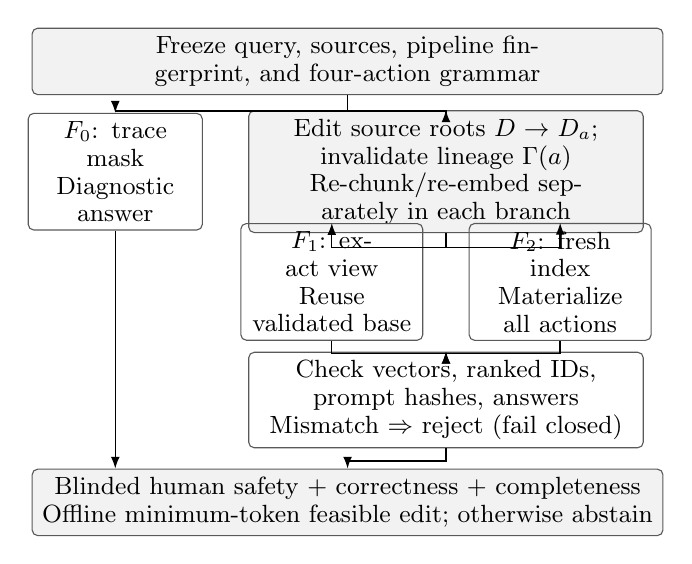
\begin{tikzpicture}[
  font=\fontsize{9}{10}\selectfont,
  box/.style={draw=black!65,rounded corners=2pt,align=center,inner sep=3pt},
  flow/.style={-{Latex[length=1.5mm]},line width=.5pt},
  x=1cm,y=1cm]
\node[box,text width=7.8cm,fill=black!5] (freeze) at (0,0)
  {Freeze query, sources, pipeline fingerprint, and four-action grammar};
\node[box,text width=2.0cm] (trace) at (-2.95,-1.4)
  {$F_0$: trace mask\\Diagnostic answer};
\node[box,text width=4.8cm,fill=black!5] (edit) at (1.25,-1.4)
  {Edit source roots $D\!\to\!D_a$; invalidate lineage $\Gamma(a)$\\Re-chunk/re-embed separately in each branch};
\node[box,text width=2.1cm] (exact) at (-.2,-2.8)
  {$F_1$: exact view\\Reuse validated base};
\node[box,text width=2.1cm] (rebuild) at (2.7,-2.8)
  {$F_2$: fresh index\\Materialize all actions};
\node[box,text width=4.8cm] (cert) at (1.25,-4.3)
  {Check vectors, ranked IDs, prompt hashes, answers\\Mismatch $\Rightarrow$ reject (fail closed)};
\node[box,text width=7.8cm,fill=black!5] (human) at (0,-5.6)
  {Blinded human safety + correctness + completeness\\Offline minimum-token feasible edit; otherwise abstain};
\draw[flow] (freeze.south) -- ++(0,-.2) -| (trace.north);
\draw[flow] (freeze.south) -- ++(0,-.2) -| (edit.north);
\draw[flow] (edit.south) -- ++(0,-.18) -| (exact.north);
\draw[flow] (edit.south) -- ++(0,-.18) -| (rebuild.north);
\draw[flow] (exact.south) -- ++(0,-.16) -| (cert.north);
\draw[flow] (rebuild.south) -- ++(0,-.16) -| (cert.north);
\draw[flow] (cert.south) -- ++(0,-.16) -| (human.north);
\draw[flow] (trace.south) -- (human.north -| trace.south);
\end{tikzpicture}

\caption{Offline repair-lattice workflow. \fzero{} diagnoses one trace; \fone{} and \ftwo{}
evaluate edited source states. All four actions are run in \ftwo{} before
human-oracle selection; certificate failure rejects a candidate.}
\label{fig:overview}
\end{figure}
\textbf{State model and repair objective.} Let $D$ be versioned source
documents and let the frozen pipeline fingerprint $\theta$ identify every
normalizer, tokenizer, chunking rule, embedding and reranking model, prompt,
and decoding parameter. Its materialized retrieval state is
\begin{equation}
 \mathcal I_\theta(D)=\operatorname{Index}_\theta(
 \operatorname{Embed}_\theta(\operatorname{Chunk}_\theta(
 \operatorname{Norm}_\theta(D)))).
\end{equation}
The output $Y(q;D,\theta)$ also includes retrieval, reranking,
prompt assembly, and generation. A source action $a$ produces $D_a$. A repair
claim is state-consistent only if it is evaluated through the same
$D_a\mapsto\mathcal I_\theta(D_a)\mapsto Y(q;D_a,\theta)$ path that will serve
after deployment. Prompt masks and vector tombstones can diagnose one trace,
but by themselves cannot establish this claim unless their counterfactual state
is shown equivalent to a source-materialized rebuild.

\textbf{Two distinct evaluation questions.} The mechanism study pairs
trace-derived repair with incident-provenance-complete quarantine, both in
\ftwo{}, to test recurrence after an apparently safe trace repair. The repair
lattice instead compares \fone{} with \ftwo{} for each of four source edits,
then selects a minimum-token human-feasible action. Provenance closure is a
matched control in the first study; exact-view equivalence is a certificate in
the second. Neither implies perfect localization.

\textbf{Root-level lineage manifest.} For each source revision $r$, the frozen
pipeline records a materialization map $L_\theta(r)$ containing its descendant
chunk and vector-entry IDs. For the source roots $A(a)$ touched by action $a$,
the invalidation set is
\begin{equation}
 \Gamma(a)=\bigcup_{r\in A(a)}L_\theta(r).
\end{equation}
Closure is essential because a deletion can change token offsets and chunk
boundaries beyond the visible sentence. Operationally, a touched source root is
the seed: we re-normalize and re-chunk the entire affected document, invalidate
its recorded old descendant IDs, and attach new descendants to the repaired
revision. This conservative root seed avoids mixing span and chunk node types.
The trace-derived arm chooses roots only from incident evidence visible in the
triggering top-5; the matched oracle control chooses every incident-owned root.
Both arms
then execute the identical rebuild code path; they differ only in provenance
coverage.

For example, deleting a sentence near a 128-token boundary can shift every
following chunk even if most characters are unchanged. Invalidating only the
visible chunk would then mix an old partition with a new source revision.
Root-level invalidation avoids this hybrid state: all old descendants of a
touched document are removed before any new descendants enter the view.
Conversely, an untouched backup document retains its validated vectors and
can rise in rank when competing poison is removed. The protocol therefore
accounts for both changed text and changed competition among unchanged text;
re-embedding just the edited span cannot represent both effects.

\textbf{Three views of one action.} \fzero{} edits the logged prompt and asks
whether the action \emph{appears} safe on the observed trace. \fone{} constructs
an exact counterfactual retrieval view without committing a new physical
index. \ftwo{} materializes the repaired corpus from source through generation
and is authoritative. For target-adoption indicator $h_t$, a repair mirage is
\begin{equation}
 M(a,q)=\mathbb 1[h_t(Y_{\rm trace}(q;a))=0\ \land\
 h_t(Y(q;D_a,\theta))=1].
\end{equation}
In the repair lattice, \fzero{} is explicitly a trace-local surrogate: it masks
the target string for span deletion, the first served incident chunk for either
sentence-level action (the hidden backup is unavailable to the trace), and all
served incident chunks for quarantine. It is not an action replay.
We report both unconditional \ftwo{} target adoption over frozen incidents and
the operational false-assurance rate conditional on initial target adoption and an
\fzero{}-safe response. This conditioning is fixed before either rebuilt
endpoint is read, and the incident remains the statistical unit.

\textbf{Counterfactual construction.} Let $E_0$ denote the labeled vectors in
the frozen index and $D_a^{\rm aff}$ the affected repaired documents. \fone{}
forms
\begin{equation}
 \widetilde E_a=(E_0\setminus\Gamma_E(a))\cup
 \operatorname{Embed}_\theta(\operatorname{Chunk}_\theta(
 \operatorname{Norm}_\theta(D_a^{\rm aff}))),
\end{equation}
where $\Gamma_E(a)$ is the vector projection of the closure. It scores the
frozen query vector against every member of $\widetilde E_a$, orders equal
scores by chunk ID, applies the frozen reranker and prompt builder, and decodes
greedily. Unchanged descendants are reused only after validating their ID,
text, and vector fingerprint bundle; every changed source is separately
re-chunked and re-embedded in each materialization. Thus the view exposes promoted backup poison and boundary-created
chunks instead of assuming that removal leaves the remainder unchanged.

\textbf{Offline closure-aware oracle analysis.} The action grammar $\mathcal A$
contains target-span deletion, visible-sentence deletion, removal of all
attack sentences, and document quarantine. For each action, \method{} performs
four deterministic steps: (1) derive $D_a^{\rm aff}$ and $\Gamma(a)$; (2)
construct $\widetilde E_a$; (3) run the complete retrieval-to-answer path in
\fone{}; and (4) record the answer, dense top-30 IDs, served top-5 IDs, edited
token count, and artifact hashes. After blinded human adjudication, the
offline oracle selects
\begin{equation}
 \begin{aligned}
 a^*_{\rm H}&=\arg\min_{a\in\mathcal A}(c(a),\tau(a))\\[-2pt]
 \mathrm{s.t.}\quad &h_t^{\rm H}(Y_{F_2})=0,\quad h_c^{\rm H}(Y_{F_2})=1,
 \quad \ell^{\rm H}(Y_{F_2})=1,
 \end{aligned}
\end{equation}
where $c(a)$ is removed-token cost and $\tau(a)$ is the lexicographic action
name recorded in the frozen manifest,
$h_c^{\rm H}$ is human correct-answer adoption, and $\ell^{\rm H}$ is human
completeness. If no candidate is feasible, the oracle records abstention. We
materialize all four actions to measure same-query feasibility and cross-engine
agreement; we do not claim a deployable semantic selector or online cost saving.

\textbf{Equivalence certificate.} \emph{Proposition 1.} If \fone{} and \ftwo{}
contain the same labeled vector multiset, share the query vector and pipeline
fingerprint, and rank exact inner products using the same chunk-ID tie-break,
then their dense rankings are identical; deterministic downstream stages yield
identical served rankings and answers. To see this, each chunk has the same
vector, label, and score in both multisets. Sorting the same score--ID pairs
gives the same dense list, after which each downstream function receives the
same ordered input. Our certificate checks chunk metadata, vector values at
absolute tolerance $10^{-6}$, exact top-30 IDs, exact top-5 served IDs, and
answer text for every action--incident pair. The tolerance is only a numerical
vector check; rank identity is certified by the exact ID comparison. The result
is query- and pipeline-specific and does not certify ANN topology, physical
erasure, unseen questions, or model weights. The paths share frozen chunking,
prompt, and generation helpers, so this is a separately materialized
cross-engine equivalence check, not an independent implementation replication.

\textbf{Protocol and failure handling.} Incidents, fingerprints, grammar,
hypotheses, and hashes are frozen first. Eligibility uses only initial and
\fzero{} labels; trace-derived and complete-lineage \ftwo{} endpoints are read
afterward. The repair lattice separately compares \fone{} with \ftwo{}; any hash,
lineage, exact-view, completeness, safety, or correctness failure rejects the
candidate. With $N$ chunks, dimension $d$, and affected source $D_a^{\rm aff}$,
screening costs $C_{\rm embed}(D_a^{\rm aff})+O(Nd)+O(N\log N)
+C_{\rm rerank}(k)+C_{\rm gen}$ per action, excluding physical serialization.

\textbf{Threat model.} An attacker may inject several external documents but
cannot modify model weights, trusted records, or the rebuild process. The
defender receives a suspected span and its source provenance. We evaluate the
repair logic under oracle provenance, then perturb locator recall and benign
false positives separately. Source localization itself is outside our claim,
and causal language is restricted to the frozen deterministic interventions in
our constructed paired design.

\textbf{State-transition invariants and audit object.} The gate requires old
and new descendant IDs to be disjoint, the unchanged-base fingerprint bundle
to match, and the two materializations to agree in source revision, chunks,
vectors, dense/served IDs, prompt hash, and answer. This distinguishes a closed
repair from local deletion followed by incomplete refresh.

Run metadata hashes the corpus, cached vectors, scripts, and model trees; each
action stores edit cost, dense/served IDs, answer, and equality checks. The
pre-annotation manifest binds all 846 blinded items, while a separate versioned
manifest binds the NumPy/FAISS certificate and server verifier without mutating
that freeze. Verifiers check fingerprints, row alignment, coverage, and
summaries and fail closed on inconsistent IDs. The complete-lineage arm is therefore
a paired experimental control: it shares the question, generator, randomness
policy, and rebuild implementation with the trace-derived arm, while changing
only incident-provenance coverage. Within these frozen constructed
interventions, this makes the endpoint the answer difference induced by
provenance closure, rather than a comparison of unrelated defenses.

\begin{figure*}[t]
\centering
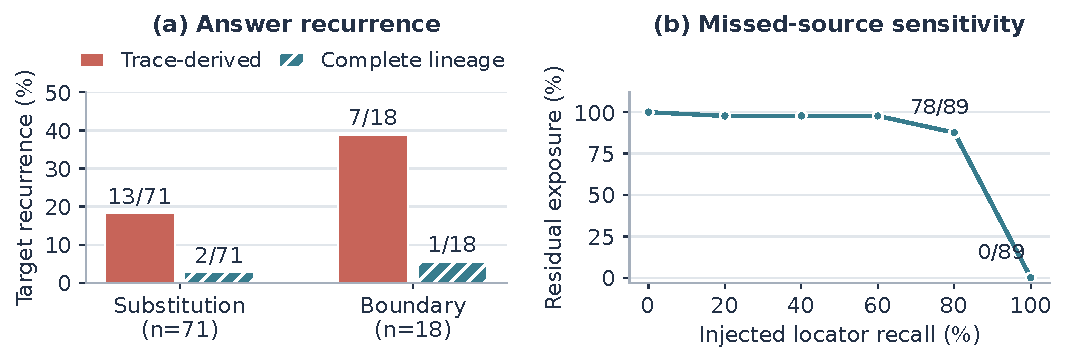
\includegraphics[width=\textwidth]{figures/main_results.pdf}
\caption{Complementary answer- and retrieval-level evaluations. (a) Adjudicated
\ftwo{} target recurrence after an \fzero{}-safe response. (b) Residual served-poison
exposure among 89 initially exposed incidents under injected source recall
with zero false positives.}
\label{fig:results}
\end{figure*}

\section{Experimental protocol}
\textbf{Frozen data.} We use the 2,681,468-document BEIR Natural Questions
corpus~\cite{thakur2021beir,kwiatkowski2019nq}. Before retrieval outcomes were observed, a hash-locked certification
set retained 94 mechanically valid synthetic incidents, each with five
separately injected poison documents. The main generator experiment uses a
100k-document snapshot containing all relevant documents, published hard
negatives, and hash-selected background documents. This is a controlled,
hard-negative-enriched stress benchmark, not a prevalence estimate.

\textbf{Pipeline and mechanisms.} BGE-base-en-v1.5~\cite{xiao2024cpack} retrieves exact top-30,
BGE-reranker-base serves top-5, and Qwen2.5-7B-Instruct~\cite{qwen2024report} generates greedily with
96 new tokens. \emph{Substitution} deletes only same-owner poison documents
visible in the initial top-5; a fresh FAISS exact index~\cite{douze2024faiss} can promote hidden
copies. \emph{Boundary migration} uses a rule frozen before outcome inspection:
one visible attack sentence is deleted from a constructed source, then the BGE
tokenizer re-chunks at 128 tokens with zero overlap; a backup target sentence
can move into a newly retrieved chunk. Both controls quarantine every
descendant of the incident source and materialize a fresh index. Corpus,
script, model-tree, and output hashes are recorded; a separate verifier
recomputes IDs, lexical labels, and summaries, and checks root-manifest
consistency.

\textbf{Labels and statistics.} The frozen flow is reported before
conditioning. Target adoption, correct-answer adoption, and truncation follow
a fixed rubric. \AnnotationStatusParagraph{} Agreement uses Cohen's
$\kappa$~\cite{cohen1960agreement}. The two mechanism tests were frozen as the
primary family in the hash-locked analysis manifest before human labels. We use
two-sided exact McNemar tests~\cite{mcnemar1947note}, Holm correction across exactly these two tests~\cite{holm1979simple},
Clopper--Pearson intervals~\cite{clopper1934limits}, and a paired 10,000-sample incident bootstrap~\cite{efron1979bootstrap} for
the main risk difference. Eligibility depends only on the initial and \fzero{}
labels, never either paired endpoint. For paired binary outcomes, the risk
difference is $(n_{10}-n_{01})/n$; resampling keeps each incident's two outcomes
together. Incomplete outputs remain in the denominator, with predeclared
directional best/worst assignments reported as sensitivity analysis.
These assignments vary only incomplete paired endpoints, holding adjudicated
initial/\fzero{} eligibility fixed; they are not worst-case bounds over
uncertain eligibility labels.

\textbf{Audit and reproducibility gates.} Every corpus snapshot, script,
model tree, annotation source, and result has a recorded SHA-256 digest. A
separate verifier reconstructs the 846 condition-blinded outputs, checks item
coverage and immutable stimulus text, verifies positional cache alignment
against the frozen corpus/query order, checks root-manifest consistency, and
recomputes summary counts. It refuses to render paper macros unless the full
hash chain and third-person decisions validate. Thus tables and figures share
one generated statistics interface rather than manually copied numbers.

\section{Results}
\textbf{Two repair-mirage mechanisms.} Table~\ref{tab:primary} reports every
conditioning step. Substitution yields \SubPartialCount{} recurrences after partial
deletion versus \SubCompleteCount{} with provenance closure; the paired difference is \SubRiskDifference{}
points (bootstrap 95\% CI \SubRiskDifferenceCI); unconditional \ftwo{} target adoption is
\SubUnconditional. The exact 95\% intervals of the two rates
are \SubPartialCI\% and \SubCompleteCI\%, respectively. Thus, even the control does not
certify risk below 5\% when its upper interval endpoint exceeds that threshold. Boundary migration yields \BoundaryPartialCount{} versus \BoundaryCompleteCount{} (intervals
\BoundaryPartialCI\% and \BoundaryCompleteCI\%). Its unconditional \ftwo{} target-adoption rate is \BoundaryUnconditional.
\PrimaryInferenceSentence

Both mechanisms rebuild from source into a fresh exact index, so neither can
be explained by stale vectors. In substitution, the removed top-5 evidence is
absent after repair and recurrence comes from a previously unserved same-owner
copy. In boundary migration, \BoundaryMechanismSentence{} The lineage-complete arm is processed
by the same code path, isolating provenance closure rather than rebuild policy.

\begin{table}[t]
\caption{Recurrence after an \fzero{}-safe response; flow is frozen
$\rightarrow$ target adopted $\rightarrow$ \fzero{} safe.}
\label{tab:primary}
\centering
\small
\begin{tabular}{lcccc}
\toprule
Mechanism & Flow & Partial & Complete & $p_{\rm Holm}$\\
\midrule
Substitution & $\SubFlow$ & \SubPartialCount & \SubCompleteCount & \SubHolm\\
Boundary & $\BoundaryFlow$ & \BoundaryPartialCount & \BoundaryCompleteCount & \BoundaryHolm\\
\bottomrule
\end{tabular}
\end{table}

\textbf{Multiplicity and locator error.} At served depth five, retrieval-level
substitution for poison multiplicity $M=1,2,3,5$ is 0, 1.1, 11.4, and 52.8\%;
therefore the main phenomenon depends on attack redundancy and disappears at
$M=1$. In a separate deterministic sensitivity sweep, 89 incidents initially
serve same-owner poison. Removing 0, 1, 2, 3, 4, or 5 of five sources leaves
89, 87, 87, 87, 78, or 0 incidents exposed (Fig.~\ref{fig:results}b). This
isolates locator recall, not a deployed locator.
A post-hoc 1M-document exact-retrieval run similarly promotes hidden poison in
49/88 initially exposed incidents (55.7\%, exact 95\% CI 44.7--66.3); it is a
retrieval-only scale check, not additional answer-level evidence.

\textbf{Utility.} On 150 frozen non-incident queries, clean and
lineage-complete corpora both retrieve a relevant document for 148/150 at
top-30 and 121/150 at top-5. The poisoned corpus is 120/150 at top-5; repair
produces one paired gain and no loss (change $+0.67$ points, bootstrap 95\% CI
0--2.0). Deterministic false-positive removal of 100/100k benign documents
changes no measured utility metric; 1000/100k causes one hit@5 loss (0.67
points). The counts preclude interpreting small decimals as broad gains.

\textbf{Repair-lattice oracle analysis.} On 30 boundary incidents, we
exhaustively evaluate target-span, visible-sentence, all-attack-sentence, and
document-quarantine actions on the triggering question. This is a feasibility
and cost oracle, not held-out generalization. A safe and correct action exists
for \RepairFeasibleCount{} (\RepairCoverage\% coverage); \RepairAbstainCount{} abstain. \RepairActionSentence{}
Separately materialized exact \fone{} and fresh-FAISS \ftwo{} paths agree for all
120 action--incident pairs in source chunks, dense and served IDs, prompt hashes,
and answers; the maximum vector discrepancy is zero. All 270 initial/\fzero{}/\ftwo{}
answers bound to human annotation remain byte-identical. Under the final
human-adjudicated labels, exact-view oracle recall is \RepairFinalistCount{} with zero token regret.
All four \ftwo{} actions were actually run for this offline oracle comparison;
no deployable semantic selector or realized online rebuild saving is claimed.
Correctness is part of feasibility: all \RepairSelectedCorrect{} selected
outputs retain it, versus \RepairDocumentCorrect{} for document quarantine. These same-query
figures must not be read as unseen-query ASR.

\textbf{Evidence boundaries.} Retrieved poison need not be adopted by the
generator; unchanged hit@5 does not establish unchanged answer quality.
Likewise, 120/120 exact-view matches certify tested questions and pipeline
states, not removal from model parameters. The 11 abstentions are not repair
successes. Hence recurrence, retrieval exposure, feasibility, and utility must
be reported separately rather than inferred from one safe masked answer.

\section{Limitations and conclusion}
The study assumes oracle provenance, one QA corpus and generator, exact dense
retrieval, and synthetic targets; the locator curve injects rather than measures
errors. Finite certification is not universal safety, human judgments remain
rubric-dependent, and the 30-case grammar is an oracle. Within these bounds,
adjudicated estimates support lineage-complete matched controls for two
constructed mechanisms; least-favorable incomplete-endpoint assignments retain
positive differences but not significance. Exact counterfactual views provide
a mechanically validated screening primitive for future deployable selectors
when their equivalence is checked rather than assumed.

Experiments use public QA and synthetic targets, without real-person targeting.

\section{Acknowledgments}
OpenAI Codex assisted research ideation, code, figures, and drafting throughout
the abstract and Sections 1--6. DeepSeek generated synthetic attacks and
auxiliary labels (Section 4); final labels came from independent human
annotation and adjudication. This disclosure does not replace author
verification or the conference's restrictions on LLM-generated manuscripts.

\clearpage
\bibliographystyle{IEEEbib}
\bibliography{refs}

\end{document}
